\chapter{Realisation}

\section*{Introduction}
Pour pouvoir mener à bien notre application mobile, il est nécessaire de choisir des technologies permettant de simplifier sa réalisation. Pour cela, et après avoir élaboré une conception détaillée des cas d’utilisation, les diagrammes de séquence, ainsi que le diagramme de classe complet dans le chapitre précédent, nous abordons la partie réalisation dans ce qui suit.

\section{Environnement de développement }
\subsection{TypeScript}
\begin{figure}[!h]
  \centering

\includegraphics[width=3cm,height=3cm,keepaspectratio]{figure/fig2.PNG}
  \caption{icon TypeScript}
\end{figure}


TypeScript est un langage open-source qui s’appuie sur JavaScript, l’un des outils les plus utilisés au monde, en ajoutant des définitions de types statiques.\\

Les types fournissent un moyen de décrire la forme d’un objet, fournissant une meilleure documentation et permettant à TypeScript de valider que votre code fonctionne correctement.


% \subsection{React Native}

% \begin{figure}[!h]
%   \centering
%   
\includegraphics[width=4cm,height=4cm,keepaspectratio]{figure/fig7.png}
%   \caption{Icon du XML }
% \end{figure}

% Un framework créé par Facebook à la suite d'un Hackaton en 2015 et une librairie Javascript développée deux ans auparavant par un ingénieur Facebook (Jordan Walke). React Native sont pratiquement identiques à ceux de React, à la différence que React Native ne manipule pas le DOM via le DOM virtuel. Il s'exécute dans un processus en arrière - plan (qui interprète le code JavaScript écrit par les développeurs) ,React Native n'utilise pas HTML. Au lieu de cela, les messages du thread JavaScript sont utilisés pour manipuler des vues natives.



% \section{Langages de programmation android }
% Il est indispensable de bien connaître Java avant de pouvoir développer pour Android, mais la plupart des développeurs utilisent également XML. Ces deux langages sont en effet recommandés par Google pour la création des applications Android.

% \newpage
\subsection{React Native}

\begin{figure}[H]
  \centering
 
\includegraphics[width=3cm,height=3cm,keepaspectratio]{figure/fig7.png}
  \caption{Icon du React Native }
\end{figure}

 Un framework créé par Facebook à la suite d'un Hackaton en 2015 et une librairie Javascript développée deux ans auparavant par un ingénieur Facebook (Jordan Walke). React Native sont pratiquement identiques à ceux de React, à la différence que React Native ne manipule pas le DOM via le DOM virtuel. Il s'exécute dans un processus en arrière - plan (qui interprète le code JavaScript écrit par les développeurs) ,React Native n'utilise pas HTML. Au lieu de cela, les messages du thread JavaScript sont utilisés pour manipuler des vues natives.


\subsection{Base de données : FireBase}

\begin{figure}[H]
  \centering
 
\includegraphics[width=3cm,height=3cm,keepaspectratio]{figure/fig2.png}
  \caption{Icon du Firebase }
\end{figure}

Firebase est un ensemble de services d'hébergement pour n'importe quel type d'application (Android, iOS, Javascript, Node.js, Java, Unity, PHP, C++ ...).\\ Il propose d'héberger en NoSQL et en temps réel des bases de données, du contenu, de l'authentification sociale (Google, Facebook, Twitter et Github), et des notifications, ou encore des services, tel que par exemple un serveur de communication temps réel.
\newpage
\subsection{Les services de Firebase}
Les services de Firebase sont : \\
\begin{figure}[H]
  \centering
 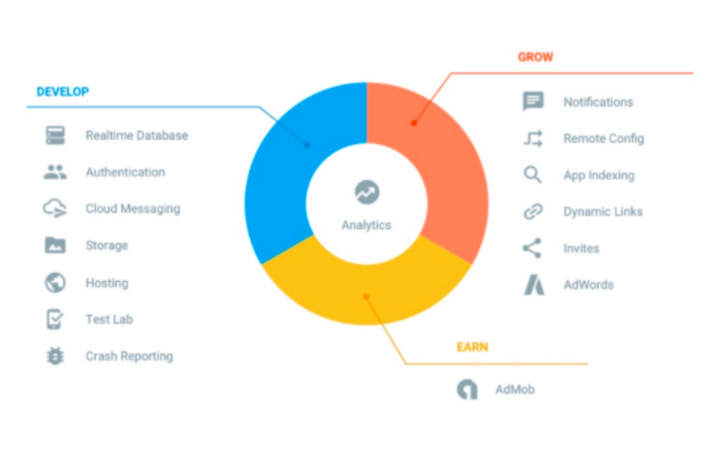
\includegraphics[width=11cm,height=11cm,keepaspectratio]{figure/fig3.png}
  \caption{Icon du sersvices de FireBase }
\end{figure}
\\
\begin{itemize}
\item Créez des applications rapidement, sans gérer l'infrastructure\\
\item Soutenu par Google, approuvé par les meilleures applications\\
\item Une plateforme, avec des produits qui fonctionnent mieux ensemble\\

\end{itemize}

% \subsection{Firebase Realtime Database}
% Firebase Realtime Database est une base de données NoSQL hébergée dans le cloud qui nous permet de stocker et de synchroniser des données entre les utilisateurs en temps réel.
% \\La synchronisation en temps réel permet à les utilisateurs d'accéder facilement à leurs données depuis n'importe quel appareil, que ce soit sur le Web ou sur un appareil mobile. La base de données en temps réel permet également à les utilisateurs de collaborer les uns avec les autres.

% Un autre gros avantage de Realtime Database est qu'elle est livrée avec des SDK mobiles et Web, nous permettant de créer vos applications sans avoir besoin de serveurs.

% \begin{figure}[h]
%   \centering

% 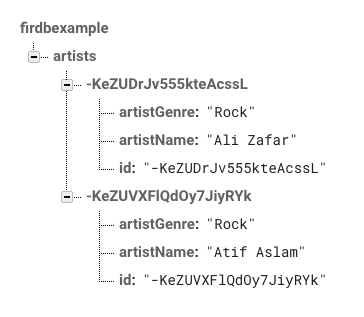
\includegraphics[width=10cm,height=10cm,keepaspectratio]{figure/fg4.png}
% \caption{example d'une base de donneés NoSQL  }
% \end{figure}
% Lorsque vos utilisateurs sont hors ligne, les SDK de base de données en temps réel utilisent le cache local sur l'appareil pour servir et stocker les modifications.\\
%  Lorsque l'appareil est en ligne, les données locales sont automatiquement synchronisées.

% \subsection{Firebase Authentication}
% \begin{figure}[h]
%   \centering
% 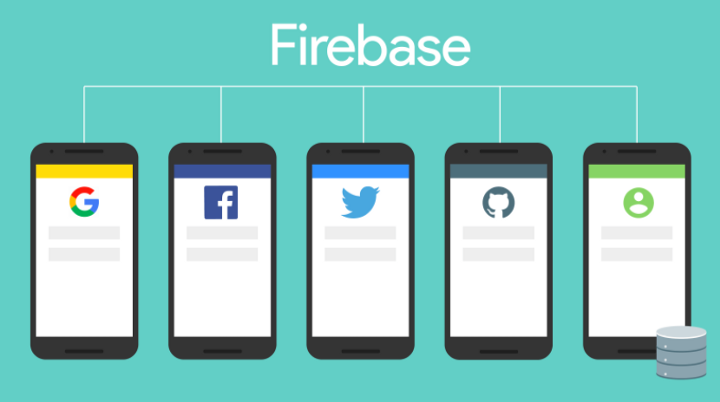
\includegraphics[width=7cm,height=5cm,keepaspectratio]{figure/fg5.png}
% \caption{Firebase Authentication}
% \end{figure}



% Firebase Authentication fournit des services backend, des SDK faciles à utiliser et des bibliothèques d'interfaces utilisateur prêtes à l'emploi pour authentifier les utilisateurs de votre application.
% \\Vous pouvez authentifier les utilisateurs de votre application à l'aide des méthodes suivantes:
% \begin{itemize}
%   \item Email et mot de passe
%   \item Numéro de téléphone
%   \item Google
%   \item Facebook
%   \item Twitter
%   \item etc !
% \end{itemize}

% L'utilisation de Firebase Authentication facilite la création de systèmes d'authentification sécurisés, tout en améliorant l'expérience de connexion et d'intégration pour les utilisateurs finaux.

% \section{La gestion du base de données}
% \subsection{Intégrez Firebase dans une application Android}

% Les projets Firebase sont des projets Google Cloud Platform qui utilisent les services Firebase et présentent les caractéristiques suivantes :

% La facturation et les autorisations relatives aux projets sont partagées entre les différentes consoles.
% Les projets qui apparaissent dans la console Firebase apparaissent également dans les consoles API Google et Google Cloud Platform.
% Lorsqu’un projet est supprimé, il est supprimé sur toutes les consoles.

% 1 – En premier lieu, si vous n’avez aucun compte Gmail, la première étape sera d’en créer un.

% 2 – Connectez-vous sur la Console Google Firebase : https://console.firebase.google.com/

% 3 – Cliquez en haut à droite sur « accéder à la console »
% \begin{figure}[h]
%   \centering
%   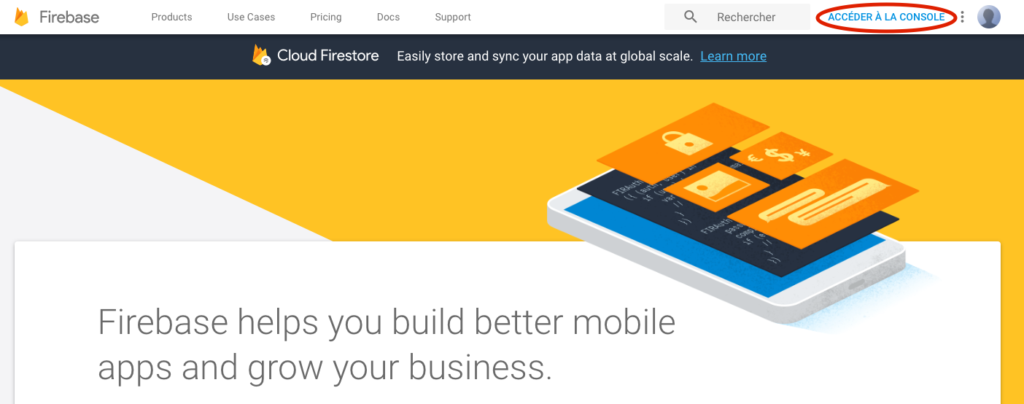
\includegraphics[width=15cm,height=10cm,keepaspectratio]{figure/fig14.png} \\
%   \caption{Interface de la page de Firebase }
% \end{figure}



% 4 – Sélectionnez le projet ou bien ajoutez un projet

% Pour ajouter un projet : Cliquer sur « ajouter un projet » cette page (photo ci-dessous) s’affiche. Il vous suffira de remplir de nom du projet et sélectionner le pays avec la liste déroulante puis cliquer sur « créer un projet »

% \begin{figure}[H]
%   \centering
%   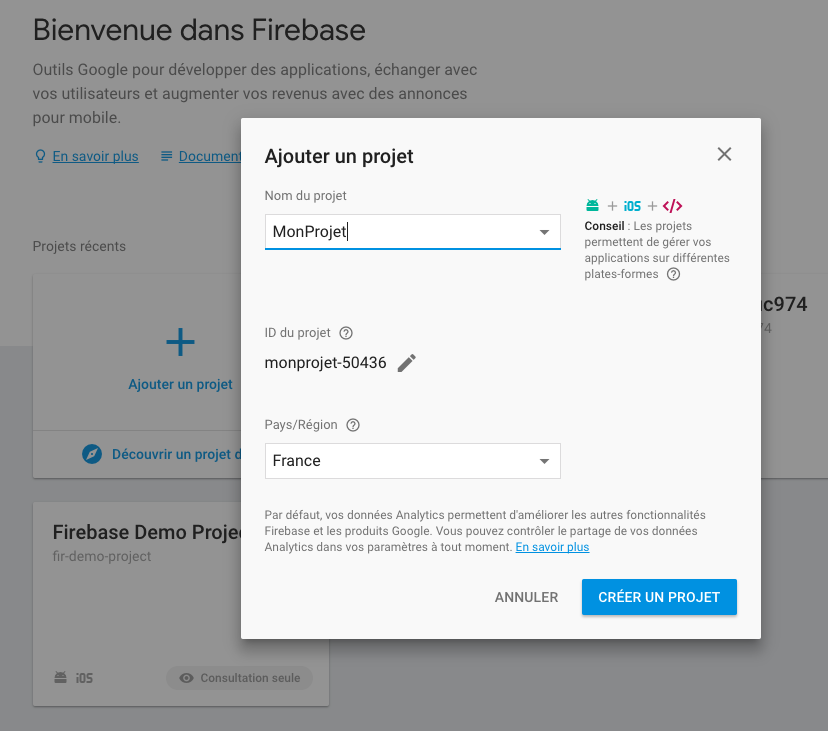
\includegraphics[width=15cm,height=10cm,keepaspectratio]{figure/fig15.png} 
% \end{figure}

% 5 – Une fois sur le projet, une nouvelle page s’affiche. Cliquez sur l’icône « Ajouter Firebase à votre application Android » (entouré en rouge sur la photo) \\

% 6 – Remplissez le « nom de package de votre application Android ». Pour cela, il faudra le demander au développeur, puis cliquez sur « Enregistrer l’application »
% \begin{center}
%   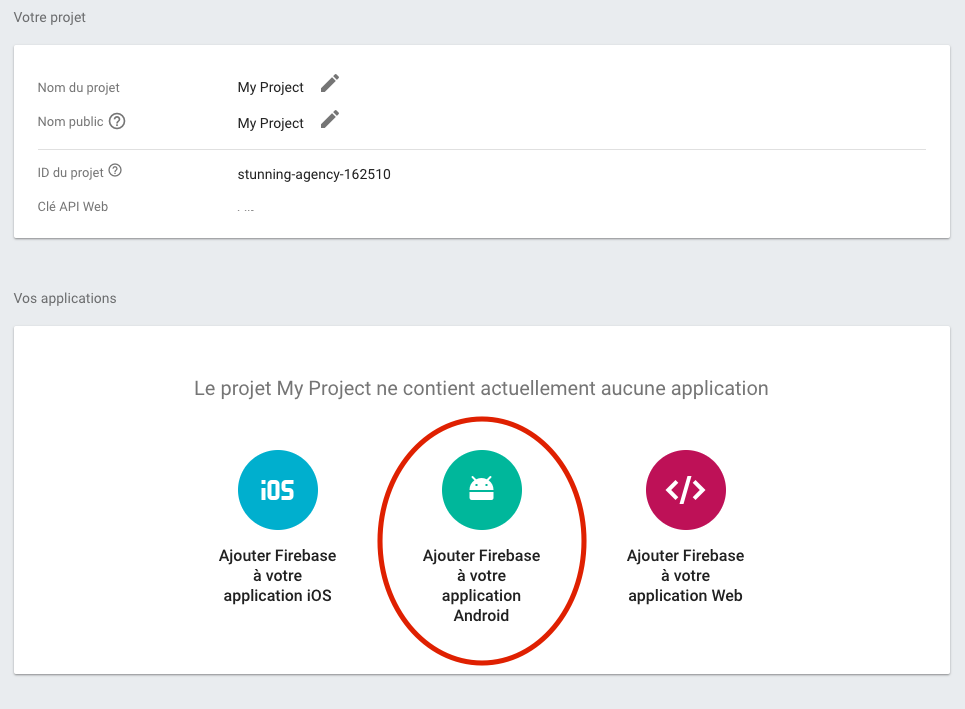
\includegraphics[width=10cm,height=10cm,keepaspectratio]{figure/fig16.png} \\
%   \end{center}


%  7 – Téléchargez le fichier « google-service-json » (gardez le fichier pour l’intégrer dans l’application) grâce au bouton et cliquez sur « Continuer »
%  \begin{center}
%   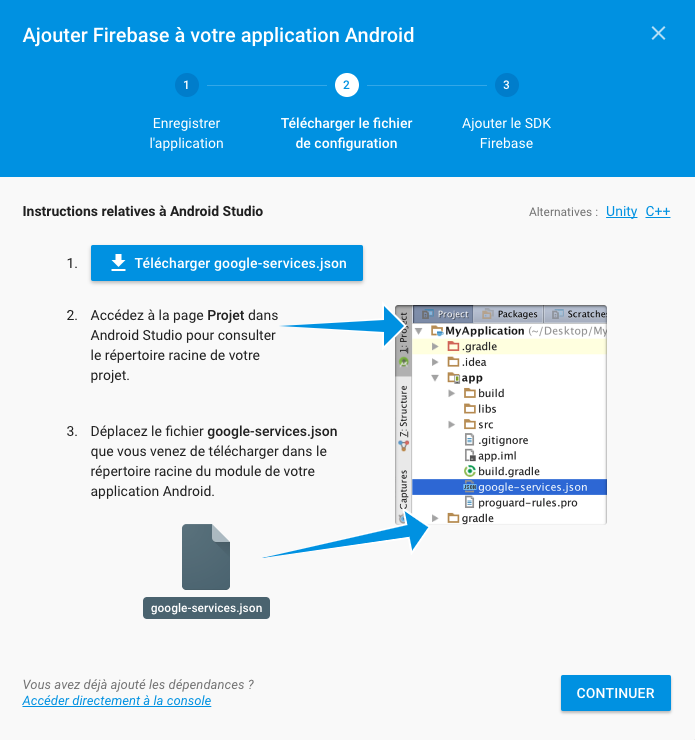
\includegraphics[width=15cm,height=10cm,keepaspectratio]{figure/fig18.png} \\
%   \end{center}

% \subsection{Structure de données}
% Sur Firebase, il existe deux types de bases de données : Firebase Realtime Database et Firebase Firestore. Ces dernières sont des bases de données dites "NoSQL" . \\
% \begin{figure}[H]
%   \centering
% 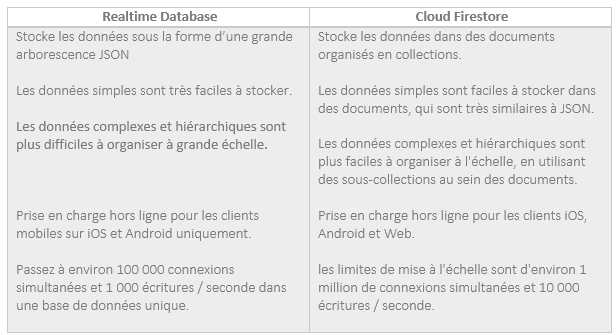
\includegraphics[width=13cm,height=15cm,keepaspectratio]{figure/fig19.png}
%   \caption{firebase realtime database vs firestore}
% \end{figure}

% \subsection{Lire et écrire des données FireBase  }
% Les données Firebase sont écrites dans une référence FirebaseDatabase et récupérées en attachant un écouteur asynchrone à la référence. L'écouteur est déclenché une fois pour l'état initial des données et à chaque fois que les données changent .
% Pour lire ou écrire des données de la base de données, vous avez besoin d'une instance de DatabaseReference:
% \begin{center}
%     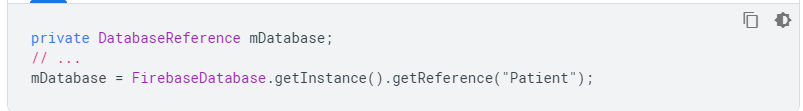
\includegraphics[width=15cm,keepaspectratio]{figure/fig21.png} \\
% \end{center}

% pour ajouter ou modifier un objet,valeur Doit être utilisé setValue ():
% \begin{center}
%     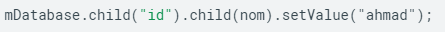
\includegraphics[width=15cm,keepaspectratio]{figure/fig22.png} \\
% \end{center}

% Pour obtenir les données,il doit définir un écouteur pour la référence. \\
% Il existe essentiellement deux types d'écouteurs que vous pouvez attacher, l'un est ValueEventListener et l'autre est ChildEventListener . Pour tout changement de données sous le nœud auquel nous avons des références et des écouteurs ajoutés, les écouteurs d'événement de valeur renvoient la structure JSON complète et l'écouteur d'événement enfant retourne un enfant spécifique où la modification s'est produite. Les deux sont utiles à leur manière. Pour extraire les données de Firebase, nous pouvons ajouter un ou plusieurs écouteurs à une référence de base de données firebase .
% Voici un exemple de code (code explicatif après code):
%     \begin{center}
%     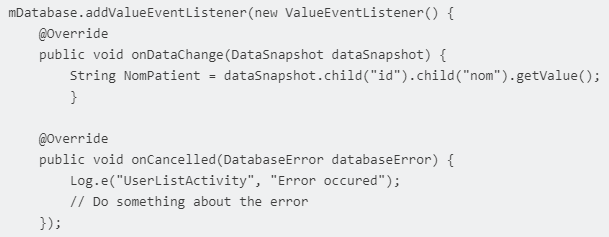
\includegraphics[width=15cm,keepaspectratio]{figure/fig23.png} \\
% \end{center}



\section*{Conclusion }
Ce chapitre contient l'ensemble des outils, framework et languages utilisés pour créer notre application.
Par la suite, nous allons à la phase de la description des interfaces graphiques de l'application. 